sections 2.5
...or had too much spin.
Physics tells that us that spin counters the translative velocity, and the boomerang slows down.
Needs reference to laws of physics.

#should be included later 

\begin{quote}
AN ODE TO A BOOMERANG TOURNEMENT\\
\\
I threw my boomerang into the air,\\
  And when it lands I know not where.\\
That’s not too swift, as you shall see,\\
  ’Cause I am throwing in accuracy.

I chucked my MTA up in the sky;\\
  It spiraled up and came out high.\\
It came in spinning with hardly a sound,\\
   And stuck the dingle arm deep in the ground.
   
I let it go with all my might,\\
  Its blazing speed was quite a sight.\\
I lined it up and reached out fast,\\
  By then my fast catch was five feet past.
  
I flicked my wrist, the boom went ’round,\\
  Coming back good but fell to the ground.\\
It bounced off my knuckles, my elbow, and thigh,\\
  Nor could I catch with my feet, I don’t know why.

Two at once is quite a chore\\
  ’Cause the old arm ends uo so sore.\\
I watch them go ’round and run to the spot,\\
  And drop left and right, as if they were hot.

I take a deep breath for throwing this round.\\
  I jump and I leap and dive to the ground.\\
I throw and I throw for a very long time,\\
 ”What do you mean I only caught nine!”

Aussie’s my favorite, I throw very long,\\
  The hook circles ’round humming its song.\\
Its sails over head, I’m followong fine,\\
  And make a diving catch over the fifty meter line.

\footnotesize \textit{Bud Pell}
\end{quote}

\begin{quote}
WHAT'S IN IT FOR ME?\\
\\
The boomerang is fun for most everyone,\\
But sometimes the purpose is lost\\
As to really what counts in the interest that mounts.\\
Is it contest, freedom, or cost?\\
\\
When you pick up the stick, and give it a flick,\\
What do you have in mind?\\
Is it beating the crowd or throwing in a shroud,\\
Or a collection from back in time?\\
\\
It’s a contest you say, the thick of the fray,\\
That keeps your interest high.\\
By taking first place, with events that you ace,\\
Puts your rang-soul up in the sky.\\
\\
Yet, throwing alone, puts a nice tone\\
On the sport of throwing the stick;\\
’Cause you don’t have to win, and, losing’s no sin--\\
It’s enjoyment that does the trick.\\
\\
And finding that boom in an old antique room,\\
A thrill for those with a yen.\\
To hang on a wall, the best booms of all,\\
And nobody will they offend.\\
\\
As I stand back and look, I could write a book\\
’Bout all the booms that I love.\\
And I think to myself, I enjoy the great wealth,\\
’Cause for me it’s all the above.\\
\footnotesize \textit{Bud Pell}
\end{quote}

\chapter{MTA and Long Distance throw}
\section{Floater and Paff III}
Correction:					& Mistake: Paff III flies straight ahead\\
									& Solution: too little or completely wrong tuning. Check again\\
									& Mistake: Paff III does not fly high\\
									& Solution: more positive dihedral on arm 1, throw harder\\
									& Mistake: Paff III flies upward and then crashes\\
									& Solution: throw at 0° or less (negative) tilt, or too much positive dihedral on both arms\\
									& Mistake: Paff III flies high, stabilizes itself and begins to swing\\
									& Solution: too much tuning, try with less tuning\\
									
\chapter{Plans}
\newpage
\section{Early Bird}
\begin{tabulary}{30em}{>{\bfseries}lL}
Shape:							& Adam ``Schlitzer'' Müller (Germany)\\
Use:								& Australian Round, Trick Catching, Throwing with wind \\
Flight distance: 			& 30 - 50 metres depending on the tuning and weight \\
Thickness/material: 	& 2 mm Fibre glass! \\
Weight: 						& 55 g / 2 oz. \vspace{0.5em} \\
Airfoil:							& 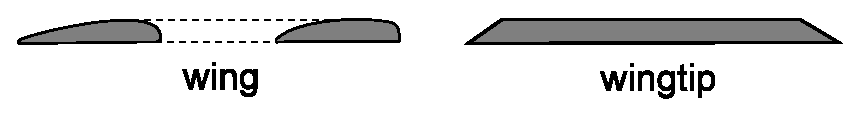
\includegraphics[width=18em]{Pictures/95_PRO16.eps} \vspace{0.5em} \\
Surface: 						& Smooth\\
Weights:						& Try attaching small coins at the wing tips\\
Tuning:						& A slight positive dihedral on the uncarved areas of the wing tips\\
Wind:							& 2 - 6 Beaufort (see Appendix on Wind force) Throw: 60° angle to the wind, 0° height of throw, 20° to 40° tilt, throw hard\\
Flight path:					& Low and very circular, slow towards the end\\
Tips:								& The Early Bird is very sensitive to tune. Small adjustments have large effects\\
\end{tabulary}
\newpage

\vspace*{\fill}
\begin{center}
	
\includegraphics[width=\textwidth]{Slowdown.eps} 
\end{center}
\vspace{\fill}

\newpage

\section{Slowdown}
\begin{tabulary}{30em}{>{\bfseries}lL}
Shape: 							& Adam ``Schlitzer'' Müller (Germany)\\
Use: 								& Accuracy \\
Flight Distance:			& 20 - 30 metres depending on the tuning \\
Thickness/material: 	& 4 mm polypropylene or wood \\
Weight: 						& 40 g / 1.4 oz. \vspace{0.5em} \\
Airfoil:							& 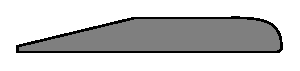
\includegraphics[width=18em]{Pictures/96_PRO17.eps} \vspace{0.5em} \\
Tuning:						& Slight positive dihedral on one or more arms and a positive angle of attack\\
Wind:							& 2 - 4 Beaufort( see Appendix on Wind force) \\
Throw:							& 90° - 100° angle to the wind, 20° - 30° hight of throw, 0° tilt, throw hard\\
Flight path: 					& A sharp rise, an elliptical flight path, a quick descent with little rotation\\
Tips: 							& The combs on the under- or topside can be taped over, to your liking\\
Special features:			& Needs plenty of wind and a strong throw\\
\end{tabulary}

\vspace*{\fill}
\begin{center}
	
\includegraphics[height=\textheight]{Tucan.eps} 
\end{center}
\vspace{\fill}

\newpage
\section{Tucan}
\begin{tabulary}{30em}{>{\bfseries}lL}
Shape:							& Earl Tutty (New Zealand)\\
Flight distance:			& 25 metres \\
Thickness/material: 	& 4 - 5 mm finnish birch plywood \\
Weight:							& 55 g / 2 oz. \vspace{0.5em} \\
Airfoil:							& 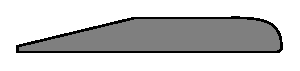
\includegraphics[width=18em]{Pictures/97_PRO18.eps} \vspace{0.5em} \\
Tuning:						& Slight positive dihedral\\
Wind: 							& 0 - 2 Beaufort (see Appendix on Wind force) \\
Throw: 							& 60° angle to the wind, 5° height of throw, 70° tilt \\
Flight Path:					& Tends to fly in an S-shape if thrown too low\\
\end{tabulary}


\vspace*{\fill}
\begin{center}
	
\includegraphics[height=\textheight]{Tern.eps} 
\end{center}
\vspace{\fill}

\newpage
\section{Tern}
\begin{tabulary}{30em}{>{\bfseries}lL}
Shape: 							& Earl Tutty (New Zealand)\\
Flight distance: 			& 25 metres \\
Thickness/material: 	& 4 mm finnish birch plywood \\
Weight: 						& 75 g / 2.7 oz. \vspace{0.5em} \\
Airfoil:							& 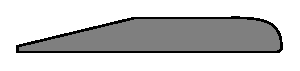
\includegraphics[width=18em]{Pictures/98_PRO19.eps} \vspace{0.5em} \\
Tuning:						& Slight positive dihedral\\
Wind: 							& 0 - 1 Beaufort (see Appendix on Wind force)\\
Throw: 							& 70° angle to the wind, 5° height of throw, 70° tilt\\
\end{tabulary}

\vspace*{\fill}
\begin{center}
	
\includegraphics[width=\textwidth]{Ghoul.eps} 
\end{center}
\vspace{\fill}		
			
\section{Ghoul}
\begin{tabulary}{30em}{>{\bfseries}lL}
Shape:							& Fridolin Frost (Germany) \\
Use: 								& Juggling, Trick Catching \\
Flight distance:			& 25 - 30 metres \\
Thickness/material:		& 4 - 5 mm finnish birch plywood\\
Weight:							& 40 g / 1.4 oz. \vspace{0.5em} \\
Airfoil:							& 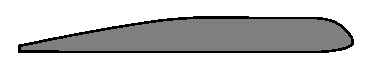
\includegraphics[width=18em]{Pictures/84_PRO5.eps} \vspace{0.5em} \\
Tuning: 						& Try very slight positive dihedral on both arms\\
Undercut: 					& Approx. 4 inch wide undercut in arm 1 and arm 2\\
Wind: 							& 0 - 2 Beaufort (see appendix on Wind force) \\
Flight path: 					& Circular, at the end of the flight path hovers high above the thrower\\
Tips: 							& Try a little weight on the underside of arm 1 and roughly parallel to the bend and possibly a flap on the topside of arm 1 or arm 2\\
\end{tabulary}
\newpage

\vspace*{\fill}
\begin{center}
	
\includegraphics[width=\textwidth]{ChallengerIII.eps} 
\end{center}
\vspace{\fill}

\newpage
\section{Challenger III}
\begin{tabulary}{30em}{>{\bfseries}lL}
Shape:							& Volker Behrens (Germany)\\
Modified by: 				& Michel Dufayard (France)\\
Use: 								& Long Distance\\
Flight distance: 			& 100 - 150 metres \\
Thickness/material: 	& 4 mm Phenolic \\
Weight: 						& 136 g / 4.9 oz fully weighted \vspace{0.5em} \\
Airfoil:							& 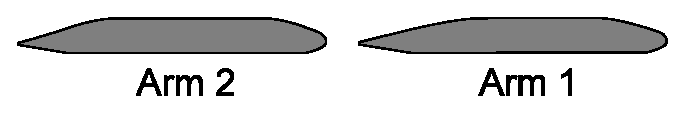
\includegraphics[width=18em]{Pictures/93_PRO14.eps} \vspace{0.5em} \\
Surface:						& Smooth\\
Weights:						& Approx. 3 g / 0.1oz.on the elbow and approx. 21 g / 0.75oz. on arm 1\\
Tuning: 						& Slight positive dihedral on arm1\\
Wind:							& 1 - 5 Beaufort (see appendix on Wind force) \\
Throw:							& 45° angle to the wind, 0° height of throw, 40° - 70° tilt, throw hard\\
Flight path:					& For the first 70 - 100 metres the boomerang flies a slight curve at a height of approx. 2 metres, rises and ``slips'' into a straight line back to the thrower. \\
Tips:								& The less undercut the trailing edge has, the shorter the flight, and easier it is to make it return. Try less weight on arm 1 at first\\
Special features:			& The present world record of 149 metres was achieved by Michel Dufayard (France)with such a model\\
\end{tabulary}

